% Chapter 3 -- Multi-Factor Models, Risk Decomposition, and Heavy-Tailed Inference
% Figures need tikz and pgfplots (with the fillbetween library) in the preamble.
\providecolor{fenavy}{HTML}{1B2A6B}
\providecolor{fegray}{HTML}{4D4D4D}

\chapter{Multi-Factor Models, Risk Decomposition, and Heavy-Tailed Inference}
\label{ch:03}

Part II of the book turns the lessons of Part I into tools. It begins with the most basic tool of all: the $t$-statistic\index{t-statistic}.

Almost every claim in quantitative finance ends in a test statistic\index{hypothesis testing!test statistic}, such as ``the strategy's alpha\index{alpha} has a $t$-statistic of 2.4.'' A $t$-statistic is an estimate, such as a mean return or an alpha, divided by its standard error\index{standard error}:
\begin{equation}
  t = \frac{\hat{\alpha}}{\operatorname{SE}(\hat{\alpha})}
  \label{eq:03-tstat}
\end{equation}
It tells us how many standard errors the estimate lies away from zero, and a value above about 1.96 is usually read as significant at the 5\% level. That reading is only as good as the standard error behind it. The usual formula for the standard error, taught in introductory statistics (see, for example, Kuo 2025), assumes that \textbf{observations are independent}, that their \textbf{spread is constant over time}, and that their \textbf{distribution is roughly normal}.

Financial returns satisfy none of these assumptions. Their tails are fat, their volatility\index{volatility} comes in clusters, and many empirical research designs build strong dependence between observations. When these assumptions fail, the standard error is often too small, so the $t$-statistic looks larger than it should, and a result can appear significant when it is not. The good news is that each of these problems has a well-tested remedy, and this chapter shows you how to choose the right one.

The $t$-statistic rarely appears alone. In most studies, the estimate on top of the fraction is an alpha from a \textbf{factor model}, a regression that explains an investment's return by its exposures to a few broad sources of risk. If the factor model leaves out a risk that the investment was paid to bear, the alpha is wrong; if the standard error ignores the features of returns, the $t$-statistic is wrong. A trustworthy claim needs both parts to be right, so this chapter develops the two together.

The claim on trial\index{claims-on-trial method} in this chapter is: \textbf{variation in expected stock returns can be explained by exposures to systematic risk factors, and regression statistics remain reliable for financial returns once standard errors account for heteroskedasticity, autocorrelation, and fat tails.} The claim has two halves. The first asks whether a small number of factors capture what drives returns. The second asks whether the statistics we use to judge those factors can be trusted.

By the end of the chapter you will be able to:
\begin{itemize}
  \item summarize a return distribution by its mean, variance, skewness, kurtosis, and autocorrelation;
  \item run and interpret linear regressions under OLS, and explain what heteroskedasticity and serial correlation do to standard errors;
  \item explain the CAPM and the Fama--French three-factor model, and interpret beta, alpha, and factor risk loadings;
  \item execute a contemporaneous linear risk decomposition, partitioning total variance into systematic factor variance and idiosyncratic residual variance;
  \item evaluate the practical and institutional implications of multi-factor architectures for asset management, style attribution, corporate finance, and macroeconomic state variable modeling;
  \item describe the stylized facts of financial returns: fat tails, volatility clustering, weak return autocorrelation, and asymmetry;
  \item choose standard errors that remain valid under these features: White, Newey--West (HAC), clustered, and Hodrick standard errors;
  \item use non-parametric block bootstrapping and Markov chain Monte Carlo (MCMC) simulations to measure uncertainty without relying on Gaussian assumptions;
  \item apply multiple-testing hurdles ($t > 3.0$) to prevent false discoveries in the factor zoo;
  \item separate statistical significance from economic significance.
\end{itemize}

In the lab you will measure these features on real data, replicate the main regressions of Fama and French (1993), compute the alphas of their 25 classic portfolios under four standard error methods, and run a controlled experiment showing how overlapping long-horizon regressions find predictability that is not there.

\section{Foundations: Distributions, Regression, and Factor Architectures}
\label{sec:03-foundations}

This section collects the tools that the rest of the chapter builds on. It starts with the numbers that describe a single return series, moves to the regression that links two series, and ends with the factor models that apply regression to the question of why some assets earn more than others. Readers who know this material can skim it, but the notation introduced here is used throughout the book.

\subsection{Describing a Distribution}
Four numbers, called \textbf{moments}, summarize a return distribution:
\begin{itemize}
  \item The \textbf{mean}\index{mean} is its center: the average return.
  \item The \textbf{variance}\index{variance|textbf}, or its square root the standard deviation\index{standard deviation}, measures spread: how far returns typically fall from the mean.
  \item \textbf{Skewness}\index{skewness|textbf} measures asymmetry. It is negative when large losses are more likely than large gains of the same size, as for most stock indexes.
  \item \textbf{Kurtosis}\index{kurtosis|textbf} measures tail heaviness. A normal distribution has kurtosis 3; values above 3 indicate \textbf{fat tails}\index{fat tails|textbf}, meaning extreme returns occur far more often than a normal distribution predicts.
\end{itemize}

Figure~\ref{fig:03-moments} shows what each moment changes, by comparing the normal distribution with one that differs in that moment alone. The first two moments are the ones most investors already use: an average return and a volatility. The last two are the ones most often ignored, and they are the ones that matter most when markets turn violent. Two portfolios can have the same mean and the same standard deviation, yet one can lose 20\% in a day far more often than the other.

\begin{figure}[htbp]
\centering
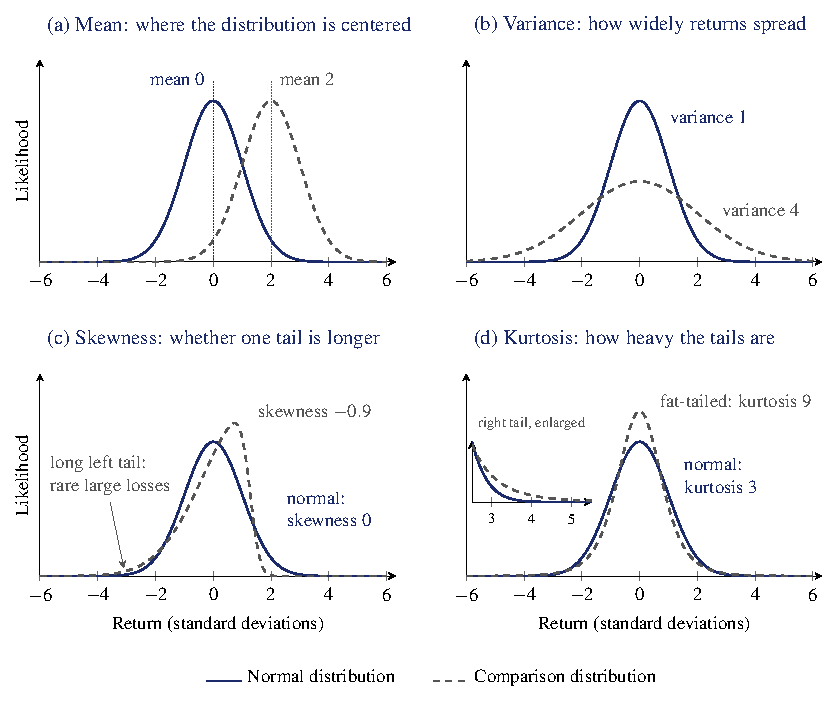
\includegraphics[width=0.7\linewidth]{images/fig03-0-moments.pdf}
\caption{The four moments of a distribution. Each panel compares the standard normal distribution (solid) with one that differs in a single respect. (a)~The mean sets the center. (b)~The variance sets the spread. (c)~Negative skewness lengthens the left tail, so large losses are more likely than large gains of the same size. (d)~Higher kurtosis puts more weight in the tails: the normal distribution has kurtosis 3, the fat-tailed one shown has kurtosis 9. Panels (c) and (d) keep the mean and variance of the normal distribution.}
\label{fig:03-moments}
\end{figure}

A fifth measure describes behavior over time. \textbf{Autocorrelation}\index{autocorrelation|textbf} is the correlation of a series with its own past values. The first-order autocorrelation ($\rho_1$) compares each month with the month before. A value near $+1$ means that a high month tends to be followed by another high month, a value near $-1$ means that it tends to be followed by a low month, and a value near zero means that the past says nothing about the next month. A return series with zero autocorrelation cannot be predicted from its own history.

\subsection{Linear Regression and OLS Assumptions}
\label{sec:03-regression}
A regression describes how a dependent variable, $y$, moves with an independent variable, $x$. Ordinary least squares\index{regression!ordinary least squares (OLS)} (OLS) fits
\begin{equation}
  y_t = \alpha + \beta x_t + \varepsilon_t
  \label{eq:03-ols}
\end{equation}
by choosing the intercept $\alpha$ and slope $\beta$ that minimize the sum of squared residuals $\sum \varepsilon_t^2$. The \textbf{residuals}\index{regression!residuals|textbf} $\varepsilon_t$ are the gaps between the actual values and the fitted line. The slope $\beta$ measures how much $y$ moves when $x$ moves by one unit, and the intercept $\alpha$ is the value of $y$ that the line predicts when $x$ is zero. The $R$-squared\index{regression!R-squared@$R^2$|textbf} ($R^2$) measures the share of the variance of $y$ explained by the regression, from 0 (none) to 1 (all).

Every estimate comes with a standard error that measures how much it would change if we drew a new sample. The classical formula for the standard error assumes that residuals are independent and identically distributed (i.i.d.) with constant variance $\sigma^2$. In words, it assumes that each residual is a fresh draw from the same distribution, unaffected by the residuals before it. Two departures from this assumption are common in finance:
\begin{itemize}
  \item \textbf{Heteroskedasticity}\index{heteroskedasticity|textbf} means that the variance of the residuals changes over time or across observations. In finance, residuals are typically small in calm years and become much larger during crises.
  \item \textbf{Serial correlation}\index{serial correlation|textbf} means that residuals are correlated with their own past values, so positive or negative errors arrive in long runs rather than alternating at random.
\end{itemize}
When either is present, OLS point estimates remain unbiased on average, but the standard analytical standard errors are wrong. They are usually too small, because the classical formula counts every observation as a separate piece of evidence, while dependent or unevenly noisy observations carry less information than they appear to.

Figure~\ref{fig:03-hetero-scatter} shows heteroskedasticity across observations, following Kuo (2025, Figure 15.4). The two panels share the same true line, but on the right the scatter of the points grows as $x$ grows. Figure~\ref{fig:03-residual-problems} shows both problems in the form they usually take in finance, which is over time. In panel~(a) the residuals become much larger during a crisis, and in panel~(b) they drift above or below zero in long runs.

\begin{figure}[!htbp]
  \centering
  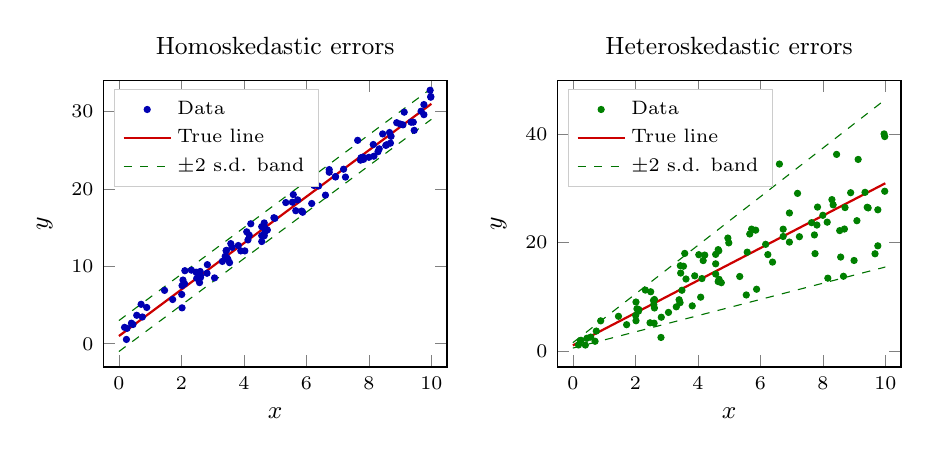
\begin{tikzpicture}
  \begin{axis}[
    name=ph,
    scale only axis, width=0.36\linewidth, height=0.3\linewidth,
    xmin=-0.5, xmax=10.5, ymin=-3, ymax=34,
    xtick={0,2,...,10},
    tick label style={font=\scriptsize}, label style={font=\small},
    xlabel={$x$}, ylabel={$y$},
    title={Homoskedastic errors}, title style={font=\small},
    legend style={font=\scriptsize, at={(0.03,0.97)}, anchor=north west, draw=gray!40},
    legend cell align=left,
  ]
    \addplot[only marks, mark=*, mark size=1.1pt, blue!70!black] coordinates {(0.18,2.12) (0.24,0.56) (0.26,1.99) (0.40,2.66) (0.45,2.49) (0.57,3.68) (0.71,5.10) (0.75,3.46) (0.89,4.69) (1.46,6.90) (1.72,5.72) (2.01,6.37) (2.02,4.64) (2.02,7.51) (2.05,8.23) (2.10,7.75) (2.11,9.44) (2.32,9.51) (2.47,9.25) (2.49,8.45) (2.58,7.90) (2.59,8.90) (2.60,9.34) (2.61,8.79) (2.61,8.56) (2.82,9.11) (2.83,10.22) (3.06,8.51) (3.31,10.64) (3.40,11.29) (3.43,12.01) (3.44,12.07) (3.45,11.16) (3.49,10.91) (3.54,10.48) (3.58,12.94) (3.62,12.46) (3.82,12.69) (3.90,12.00) (4.03,12.00) (4.09,14.46) (4.13,13.42) (4.17,14.03) (4.22,15.50) (4.57,13.21) (4.57,13.97) (4.57,15.13) (4.65,15.61) (4.65,13.95) (4.67,14.97) (4.68,14.47) (4.75,14.70) (4.96,16.28) (4.99,16.20) (5.34,18.24) (5.55,18.29) (5.58,19.27) (5.66,17.19) (5.72,18.59) (5.85,17.14) (5.88,16.99) (6.17,18.12) (6.24,20.45) (6.39,20.38) (6.61,19.20) (6.73,22.50) (6.73,22.16) (6.93,21.60) (6.93,21.55) (7.19,22.55) (7.25,21.53) (7.64,26.28) (7.73,23.72) (7.75,24.04) (7.81,24.12) (7.83,23.83) (8.00,24.09) (8.14,25.74) (8.16,24.23) (8.29,24.81) (8.33,25.18) (8.44,27.11) (8.54,25.63) (8.57,25.71) (8.66,27.29) (8.69,25.92) (8.71,26.80) (8.89,28.56) (9.00,28.39) (9.09,28.28) (9.13,29.92) (9.35,28.62) (9.42,28.63) (9.45,27.57) (9.67,30.04) (9.76,30.90) (9.76,29.60) (9.96,32.75) (9.98,31.95) (9.98,31.85)};
    \addlegendentry{Data}
    \addplot[red!80!black, thick, domain=0:10, samples=2] {1+3*x};
    \addlegendentry{True line}
    \addplot[green!45!black, dashed, domain=0:10, samples=2] {1+3*x+2};
    \addlegendentry{$\pm 2$ s.d. band}
    \addplot[green!45!black, dashed, domain=0:10, samples=2, forget plot] {1+3*x-2};
  \end{axis}
  \begin{axis}[
    at={(ph.east)}, anchor=west, xshift=1.4cm,
    name=pt,
    scale only axis, width=0.36\linewidth, height=0.3\linewidth,
    xmin=-0.5, xmax=10.5, ymin=-3, ymax=50,
    xtick={0,2,...,10},
    tick label style={font=\scriptsize}, label style={font=\small},
    xlabel={$x$}, ylabel={$y$},
    title={Heteroskedastic errors}, title style={font=\small},
    legend style={font=\scriptsize, at={(0.03,0.97)}, anchor=north west, draw=gray!40},
    legend cell align=left,
  ]
    \addplot[only marks, mark=*, mark size=1.1pt, green!50!black] coordinates {(0.18,1.08) (0.24,1.85) (0.26,1.94) (0.40,1.06) (0.45,2.32) (0.57,2.53) (0.71,1.76) (0.75,3.65) (0.89,5.54) (1.46,6.38) (1.72,4.83) (2.01,6.54) (2.02,9.02) (2.02,5.56) (2.05,7.77) (2.10,7.33) (2.11,7.63) (2.32,11.23) (2.47,5.18) (2.49,10.92) (2.58,9.31) (2.59,8.54) (2.60,5.11) (2.61,9.49) (2.61,7.92) (2.82,2.47) (2.83,6.21) (3.06,7.10) (3.31,8.13) (3.40,9.44) (3.43,8.90) (3.44,15.74) (3.45,14.38) (3.49,11.20) (3.54,15.65) (3.58,18.02) (3.62,13.28) (3.82,8.31) (3.90,13.87) (4.03,17.78) (4.09,9.92) (4.13,13.36) (4.17,16.69) (4.22,17.71) (4.57,17.84) (4.57,16.09) (4.57,14.20) (4.65,12.81) (4.65,18.72) (4.67,18.50) (4.68,13.21) (4.75,12.60) (4.96,20.86) (4.99,19.97) (5.34,13.75) (5.55,10.33) (5.58,18.25) (5.66,21.61) (5.72,22.51) (5.85,22.32) (5.88,11.39) (6.17,19.70) (6.24,17.80) (6.39,16.41) (6.61,34.55) (6.73,21.15) (6.73,22.50) (6.93,20.11) (6.93,25.50) (7.19,29.13) (7.25,21.11) (7.64,23.71) (7.73,21.44) (7.75,17.98) (7.81,23.27) (7.83,26.59) (8.00,25.07) (8.14,23.80) (8.16,13.44) (8.29,27.97) (8.33,27.00) (8.44,36.34) (8.54,22.24) (8.57,17.34) (8.66,13.79) (8.69,22.53) (8.71,26.50) (8.89,29.25) (9.00,16.71) (9.09,24.07) (9.13,35.41) (9.35,29.32) (9.42,26.56) (9.45,26.44) (9.67,17.95) (9.76,19.42) (9.76,26.09) (9.96,40.13) (9.98,39.64) (9.98,29.52)};
    \addlegendentry{Data}
    \addplot[red!80!black, thick, domain=0:10, samples=2] {1+3*x};
    \addlegendentry{True line}
    \addplot[green!45!black, dashed, domain=0:10, samples=2] {(1+3*x)*1.5};
    \addlegendentry{$\pm 2$ s.d. band}
    \addplot[green!45!black, dashed, domain=0:10, samples=2, forget plot] {(1+3*x)*0.5};
  \end{axis}
  \end{tikzpicture}
  \caption{Homoskedastic and heteroskedastic errors around the same true line, $y = 1 + 3x$, shown with simulated data. On the left, the scatter around the line has the same width everywhere, so the dashed bands run parallel to the line. On the right, the scatter grows with $x$, so the bands fan out. The fitted line is unbiased in both cases, but on the right the usual standard error understates the uncertainty. After Kuo (2025, Figure 15.4).}
  \label{fig:03-hetero-scatter}
\end{figure}

\begin{figure}[!htbp]
  \centering
  \begin{tikzpicture}
  % Panel (a): heteroskedasticity
  \begin{axis}[
    name=pa,
    scale only axis, width=0.55\linewidth, height=0.17\linewidth,
    axis lines=left, axis line style={-stealth, thin},
    xmin=0, xmax=205, ymin=-7.5, ymax=7.5,
    xtick=\empty, ytick={-5,0,5},
    tick label style={font=\small}, label style={font=\small},
    ylabel={Residual},
    title={(a) Heteroskedasticity: the spread changes},
    title style={font=\small, anchor=south west, at={(0,1)}, xshift=-4pt},
    clip=false,
  ]
    % Plus or minus two standard deviations
    \addplot[name path=up, gray!60, thin] coordinates {(1,2.00) (2,2.00) (3,2.00) (4,2.00) (5,2.00) (6,2.00) (7,2.00) (8,2.00) (9,2.00) (10,2.00) (11,2.00) (12,2.00) (13,2.00) (14,2.00) (15,2.00) (16,2.00) (17,2.00) (18,2.00) (19,2.00) (20,2.00) (21,2.00) (22,2.00) (23,2.00) (24,2.00) (25,2.00) (26,2.00) (27,2.00) (28,2.00) (29,2.00) (30,2.00) (31,2.00) (32,2.00) (33,2.00) (34,2.00) (35,2.00) (36,2.00) (37,2.00) (38,2.00) (39,2.00) (40,2.00) (41,2.00) (42,2.00) (43,2.00) (44,2.00) (45,2.00) (46,2.00) (47,2.00) (48,2.00) (49,2.00) (50,2.00) (51,2.00) (52,2.00) (53,2.00) (54,2.00) (55,2.00) (56,2.00) (57,2.00) (58,2.00) (59,2.00) (60,2.00) (61,2.00) (62,2.00) (63,2.00) (64,2.00) (65,2.00) (66,2.00) (67,2.00) (68,2.00) (69,2.00) (70,2.00) (71,2.00) (72,2.00) (73,2.00) (74,2.00) (75,2.00) (76,2.00) (77,2.00) (78,2.00) (79,2.00) (80,2.00) (81,2.00) (82,2.00) (83,2.00) (84,2.00) (85,2.00) (86,2.00) (87,2.00) (88,2.00) (89,2.00) (90,2.00) (91,2.00) (92,2.00) (93,2.00) (94,2.00) (95,2.00) (96,2.00) (97,2.00) (98,2.00) (99,2.00) (100,2.00) (101,2.00) (102,2.00) (103,2.00) (104,2.00) (105,2.00) (106,2.00) (107,2.57) (108,3.14) (109,3.71) (110,4.29) (111,4.86) (112,5.43) (113,6.00) (114,6.00) (115,6.00) (116,6.00) (117,6.00) (118,6.00) (119,6.00) (120,6.00) (121,6.00) (122,6.00) (123,6.00) (124,6.00) (125,6.00) (126,6.00) (127,6.00) (128,6.00) (129,6.00) (130,6.00) (131,6.00) (132,6.00) (133,6.00) (134,6.00) (135,6.00) (136,6.00) (137,6.00) (138,5.43) (139,4.86) (140,4.29) (141,3.71) (142,3.14) (143,2.57) (144,2.00) (145,2.00) (146,2.00) (147,2.00) (148,2.00) (149,2.00) (150,2.00) (151,2.00) (152,2.00) (153,2.00) (154,2.00) (155,2.00) (156,2.00) (157,2.00) (158,2.00) (159,2.00) (160,2.00) (161,2.00) (162,2.00) (163,2.00) (164,2.00) (165,2.00) (166,2.00) (167,2.00) (168,2.00) (169,2.00) (170,2.00) (171,2.00) (172,2.00) (173,2.00) (174,2.00) (175,2.00) (176,2.00) (177,2.00) (178,2.00) (179,2.00) (180,2.00) (181,2.00) (182,2.00) (183,2.00) (184,2.00) (185,2.00) (186,2.00) (187,2.00) (188,2.00) (189,2.00) (190,2.00) (191,2.00) (192,2.00) (193,2.00) (194,2.00) (195,2.00) (196,2.00) (197,2.00) (198,2.00) (199,2.00) (200,2.00)};
    \addplot[name path=lo, gray!60, thin] coordinates {(1,-2.00) (2,-2.00) (3,-2.00) (4,-2.00) (5,-2.00) (6,-2.00) (7,-2.00) (8,-2.00) (9,-2.00) (10,-2.00) (11,-2.00) (12,-2.00) (13,-2.00) (14,-2.00) (15,-2.00) (16,-2.00) (17,-2.00) (18,-2.00) (19,-2.00) (20,-2.00) (21,-2.00) (22,-2.00) (23,-2.00) (24,-2.00) (25,-2.00) (26,-2.00) (27,-2.00) (28,-2.00) (29,-2.00) (30,-2.00) (31,-2.00) (32,-2.00) (33,-2.00) (34,-2.00) (35,-2.00) (36,-2.00) (37,-2.00) (38,-2.00) (39,-2.00) (40,-2.00) (41,-2.00) (42,-2.00) (43,-2.00) (44,-2.00) (45,-2.00) (46,-2.00) (47,-2.00) (48,-2.00) (49,-2.00) (50,-2.00) (51,-2.00) (52,-2.00) (53,-2.00) (54,-2.00) (55,-2.00) (56,-2.00) (57,-2.00) (58,-2.00) (59,-2.00) (60,-2.00) (61,-2.00) (62,-2.00) (63,-2.00) (64,-2.00) (65,-2.00) (66,-2.00) (67,-2.00) (68,-2.00) (69,-2.00) (70,-2.00) (71,-2.00) (72,-2.00) (73,-2.00) (74,-2.00) (75,-2.00) (76,-2.00) (77,-2.00) (78,-2.00) (79,-2.00) (80,-2.00) (81,-2.00) (82,-2.00) (83,-2.00) (84,-2.00) (85,-2.00) (86,-2.00) (87,-2.00) (88,-2.00) (89,-2.00) (90,-2.00) (91,-2.00) (92,-2.00) (93,-2.00) (94,-2.00) (95,-2.00) (96,-2.00) (97,-2.00) (98,-2.00) (99,-2.00) (100,-2.00) (101,-2.00) (102,-2.00) (103,-2.00) (104,-2.00) (105,-2.00) (106,-2.00) (107,-2.57) (108,-3.14) (109,-3.71) (110,-4.29) (111,-4.86) (112,-5.43) (113,-6.00) (114,-6.00) (115,-6.00) (116,-6.00) (117,-6.00) (118,-6.00) (119,-6.00) (120,-6.00) (121,-6.00) (122,-6.00) (123,-6.00) (124,-6.00) (125,-6.00) (126,-6.00) (127,-6.00) (128,-6.00) (129,-6.00) (130,-6.00) (131,-6.00) (132,-6.00) (133,-6.00) (134,-6.00) (135,-6.00) (136,-6.00) (137,-6.00) (138,-5.43) (139,-4.86) (140,-4.29) (141,-3.71) (142,-3.14) (143,-2.57) (144,-2.00) (145,-2.00) (146,-2.00) (147,-2.00) (148,-2.00) (149,-2.00) (150,-2.00) (151,-2.00) (152,-2.00) (153,-2.00) (154,-2.00) (155,-2.00) (156,-2.00) (157,-2.00) (158,-2.00) (159,-2.00) (160,-2.00) (161,-2.00) (162,-2.00) (163,-2.00) (164,-2.00) (165,-2.00) (166,-2.00) (167,-2.00) (168,-2.00) (169,-2.00) (170,-2.00) (171,-2.00) (172,-2.00) (173,-2.00) (174,-2.00) (175,-2.00) (176,-2.00) (177,-2.00) (178,-2.00) (179,-2.00) (180,-2.00) (181,-2.00) (182,-2.00) (183,-2.00) (184,-2.00) (185,-2.00) (186,-2.00) (187,-2.00) (188,-2.00) (189,-2.00) (190,-2.00) (191,-2.00) (192,-2.00) (193,-2.00) (194,-2.00) (195,-2.00) (196,-2.00) (197,-2.00) (198,-2.00) (199,-2.00) (200,-2.00)};
    \addplot[fenavy!12] fill between[of=up and lo];
    \draw[gray!70, thin] (axis cs:0,0) -- (axis cs:200,0);
    \addplot[fenavy, thin, mark=none] coordinates {(1,0.00) (2,0.30) (3,-0.27) (4,-0.89) (5,-0.45) (6,-0.99) (7,0.06) (8,1.34) (9,-0.49) (10,-0.62) (11,0.49) (12,0.36) (13,0.11) (14,-0.93) (15,-0.03) (16,0.70) (17,-1.34) (18,-0.46) (19,-1.90) (20,-1.29) (21,-1.84) (22,-0.24) (23,-1.27) (24,0.27) (25,0.16) (26,-0.19) (27,-2.52) (28,-0.54) (29,-0.05) (30,0.11) (31,-1.53) (32,-0.48) (33,-0.98) (34,-0.81) (35,1.06) (36,-0.81) (37,-0.03) (38,0.88) (39,-0.58) (40,-0.11) (41,0.11) (42,0.06) (43,-1.23) (44,0.08) (45,1.36) (46,-1.55) (47,0.86) (48,0.12) (49,-0.64) (50,2.00) (51,0.76) (52,-1.20) (53,0.07) (54,0.58) (55,-0.19) (56,0.68) (57,-0.07) (58,0.67) (59,1.44) (60,-0.68) (61,0.20) (62,-0.46) (63,0.13) (64,-1.19) (65,-0.58) (66,-0.20) (67,0.90) (68,1.15) (69,-1.32) (70,-0.79) (71,0.65) (72,-1.99) (73,-0.46) (74,-0.10) (75,1.26) (76,0.69) (77,-0.33) (78,-0.37) (79,-0.25) (80,1.52) (81,-0.43) (82,-0.30) (83,0.35) (84,-0.12) (85,-0.20) (86,-1.11) (87,-0.01) (88,-0.44) (89,1.17) (90,0.65) (91,-0.02) (92,0.67) (93,-0.34) (94,1.05) (95,-0.01) (96,0.58) (97,-1.29) (98,0.35) (99,-1.69) (100,-2.04) (101,-0.30) (102,-0.90) (103,0.16) (104,2.24) (105,-0.83) (106,-0.62) (107,0.26) (108,0.77) (109,-0.33) (110,-0.44) (111,1.71) (112,1.41) (113,-3.10) (114,-0.24) (115,0.11) (116,-3.16) (117,0.78) (118,-2.57) (119,2.92) (120,0.58) (121,0.27) (122,-1.77) (123,-0.36) (124,-5.99) (125,-3.39) (126,1.09) (127,-6.39) (128,2.54) (129,-5.24) (130,2.27) (131,-2.54) (132,2.34) (133,0.39) (134,-4.61) (135,3.75) (136,4.33) (137,-0.20) (138,-0.74) (139,-0.39) (140,-2.09) (141,2.04) (142,-0.85) (143,-0.07) (144,-0.79) (145,-0.63) (146,-1.28) (147,1.26) (148,-0.15) (149,0.97) (150,0.01) (151,-0.69) (152,-0.33) (153,-0.56) (154,0.01) (155,-0.38) (156,-0.30) (157,-1.38) (158,-0.81) (159,1.65) (160,-0.67) (161,-1.05) (162,0.34) (163,1.41) (164,-1.45) (165,-0.21) (166,-0.63) (167,-1.76) (168,0.73) (169,-0.02) (170,0.07) (171,-0.75) (172,0.45) (173,-0.54) (174,-0.14) (175,-1.11) (176,-1.22) (177,1.34) (178,-0.51) (179,0.29) (180,-0.03) (181,-0.44) (182,-0.51) (183,0.63) (184,-0.30) (185,-0.15) (186,0.02) (187,1.18) (188,0.68) (189,0.38) (190,-0.56) (191,-1.38) (192,0.95) (193,0.97) (194,-0.14) (195,0.54) (196,0.78) (197,0.83) (198,0.92) (199,-0.46) (200,1.51)};
    \node[font=\footnotesize, anchor=south] at (axis cs:125,6.2) {crisis: large errors};
    \node[font=\footnotesize, anchor=south, gray!60!black] at (axis cs:50,2.6) {calm: small errors};
  \end{axis}

  % Panel (b): serial correlation
  \begin{axis}[
    at={(pa.south west)}, anchor=north west, yshift=-1.1cm,
    scale only axis, width=0.55\linewidth, height=0.17\linewidth,
    axis lines=left, axis line style={-stealth, thin},
    xmin=0, xmax=205, ymin=-4.5, ymax=4.5,
    xtick=\empty, ytick={-3,0,3},
    tick label style={font=\small}, label style={font=\small},
    xlabel={Time}, ylabel={Residual},
    title={(b) Serial correlation: errors come in runs},
    title style={font=\small, anchor=south west, at={(0,1)}, xshift=-4pt},
    clip=false,
  ]
    \draw[gray!70, thin] (axis cs:0,0) -- (axis cs:200,0);
    \addplot[fenavy, thin, mark=none] coordinates {(1,0.18) (2,0.60) (3,0.77) (4,1.12) (5,1.94) (6,2.43) (7,1.46) (8,0.35) (9,0.73) (10,0.09) (11,0.07) (12,0.50) (13,-0.44) (14,-1.49) (15,-1.13) (16,-0.93) (17,-0.92) (18,-0.77) (19,-1.10) (20,-1.74) (21,-1.56) (22,-1.84) (23,-2.43) (24,-1.80) (25,-1.56) (26,-1.11) (27,-1.47) (28,-1.59) (29,-1.88) (30,-2.07) (31,-1.65) (32,-1.82) (33,-1.36) (34,-0.97) (35,0.24) (36,-0.53) (37,0.02) (38,-0.03) (39,-0.04) (40,-0.79) (41,-0.92) (42,-0.39) (43,-0.37) (44,-0.27) (45,-0.39) (46,0.28) (47,0.23) (48,-0.97) (49,-1.19) (50,-2.05) (51,-3.45) (52,-3.21) (53,-2.03) (54,-1.70) (55,-2.06) (56,-2.25) (57,-1.32) (58,-1.04) (59,-0.85) (60,-0.75) (61,-0.62) (62,-0.10) (63,0.20) (64,0.29) (65,-0.31) (66,0.01) (67,-0.35) (68,0.28) (69,-0.43) (70,-0.44) (71,-0.38) (72,-1.02) (73,0.04) (74,0.80) (75,0.44) (76,0.78) (77,0.86) (78,-0.64) (79,-0.42) (80,-0.39) (81,-0.28) (82,-0.81) (83,-0.83) (84,-0.80) (85,-0.05) (86,0.13) (87,0.11) (88,0.90) (89,0.47) (90,0.19) (91,-0.79) (92,0.15) (93,0.64) (94,1.03) (95,1.22) (96,1.10) (97,1.05) (98,0.76) (99,0.54) (100,0.48) (101,1.21) (102,1.32) (103,1.09) (104,0.62) (105,0.19) (106,1.01) (107,1.13) (108,0.99) (109,0.66) (110,-0.02) (111,-0.05) (112,0.41) (113,0.15) (114,0.00) (115,-0.11) (116,-0.04) (117,-0.87) (118,-0.87) (119,-1.19) (120,-0.54) (121,-0.87) (122,-0.43) (123,0.44) (124,0.20) (125,-0.14) (126,-0.02) (127,-0.02) (128,-0.54) (129,-0.22) (130,0.88) (131,0.61) (132,0.41) (133,-0.20) (134,-0.00) (135,-0.66) (136,-1.14) (137,-0.30) (138,-0.73) (139,-0.05) (140,0.76) (141,0.78) (142,0.96) (143,1.84) (144,1.46) (145,0.93) (146,0.08) (147,0.09) (148,0.85) (149,1.23) (150,0.55) (151,0.02) (152,-0.25) (153,-0.06) (154,-0.16) (155,-0.02) (156,0.14) (157,-0.04) (158,-0.06) (159,0.06) (160,0.01) (161,0.27) (162,1.22) (163,1.35) (164,1.17) (165,0.11) (166,0.30) (167,-0.77) (168,-1.40) (169,-0.74) (170,-0.26) (171,-0.30) (172,-1.15) (173,-1.18) (174,-1.36) (175,-0.82) (176,0.49) (177,0.53) (178,0.04) (179,-0.58) (180,-0.52) (181,-0.54) (182,-1.06) (183,-0.84) (184,-1.32) (185,-0.54) (186,0.10) (187,0.66) (188,0.31) (189,0.53) (190,0.38) (191,0.12) (192,-0.07) (193,-0.75) (194,-1.40) (195,-0.77) (196,-0.75) (197,-0.53) (198,0.08) (199,-0.85) (200,-1.13)};
  \end{axis}
  \end{tikzpicture}
  \caption{Two ways regression residuals break the textbook assumptions, shown with simulated data. In panel~(a) the errors are independent, but their spread, shown by the shaded band of plus or minus two standard deviations, triples during a crisis. In panel~(b) the spread is constant, but each error is strongly correlated with the one before it, so positive and negative errors arrive in long runs. In both cases the usual standard error is wrong.}
  \label{fig:03-residual-problems}
\end{figure}

\subsection{The Capital Asset Pricing Model (CAPM)}
\label{sec:03-capm}
The Capital Asset Pricing Model\index{capital asset pricing model (CAPM)} (Sharpe 1964, Lintner 1965, Mossin 1966) splits risk into two components. \textbf{Systematic risk}\index{risk!systematic|textbf} moves with the aggregate market and cannot be diversified away. \textbf{Idiosyncratic risk}\index{risk!idiosyncratic|textbf} is unique to individual assets and can be eliminated by holding a broad portfolio, a practice called \textbf{diversification}\index{diversification|textbf}. Because investors can remove idiosyncratic risk at almost no cost, the model says that they should not expect to be paid for bearing it. Only systematic risk earns a reward.

This one idea still underlies almost all of asset pricing, and its reach into practice is wide. Companies use the CAPM to set the discount rate\index{discount rate} for investment projects, and surveys find that most finance officers rely on it to estimate their cost of capital (Graham and Harvey 2001). The idea of alpha, the return beyond what market exposure explains, comes directly from the model, and its conclusion that the market portfolio is the best risky portfolio for every investor gave index funds their theoretical foundation.

Formally, the CAPM says that an asset's expected excess return\index{return!excess} is proportional to its \textbf{beta}\index{beta|textbf}, its sensitivity to the market:
\begin{equation}
  E[R_i] - r_f = \beta_i \left(E[R_m] - r_f\right), \qquad \beta_i = \frac{\operatorname{Cov}(R_i, R_m)}{\operatorname{Var}(R_m)}
  \label{eq:03-capm}
\end{equation}
Here $R_i$ is the asset's return, $R_m$ the market's return, and $r_f$ the risk-free rate. The covariance $\operatorname{Cov}$ measures how two returns move together, and the variance $\operatorname{Var}$ measures how much one return moves on its own. A stock with a beta of 1.5 tends to rise 1.5\% when the market rises 1\%, so it carries one and a half times the market's systematic risk and should earn one and a half times the market's excess return.

The regression model is estimated in time series:
\begin{equation}
  R_{i,t} - r_{f,t} = \alpha_i + \beta_i (R_{m,t} - r_{f,t}) + \varepsilon_{i,t}
  \label{eq:03-capm-ts}
\end{equation}
This is Equation~\eqref{eq:03-ols} with the asset's excess return as $y$ and the market's excess return as $x$. The slope $\beta_i$ measures systematic market sensitivity. The intercept $\alpha_i$\index{alpha|textbf} (alpha) represents the average excess return that market exposure does not explain. The model predicts that $\alpha_i = 0$ for all assets, so a positive alpha is either evidence against the model or evidence of skill. Figure~\ref{fig:03-alpha} shows the two numbers on a scatter plot.

\begin{figure}[!htbp]
  \centering
  \begin{tikzpicture}[
    % Fitted regression: strategy = 1.16 + 1.15 * market
    declare function={fit(\x) = 1.16 + 1.15*\x;  zero(\x) = 1.15*\x;}
  ]
  \begin{axis}[
    scale only axis, width=0.41\linewidth, height=0.29\linewidth,
    axis lines=left,
    axis line style={-stealth, thin},
    xmin=-11, xmax=12.5, ymin=-12.5, ymax=16,
    xtick={-8,-4,0,4,8,12},
    ytick={-10,-5,0,5,10,15},
    tick label style={font=\footnotesize}, label style={font=\small},
    xlabel={Market excess return, $R_m - r_f$ (\% a month)},
    ylabel={Strategy excess return (\%)},
    clip=false,
  ]
    % Reference axes through zero
    \draw[gray!40] (axis cs:-11,0) -- (axis cs:12.5,0);
    \draw[gray!40] (axis cs:0,-12.5) -- (axis cs:0,16);

    % Monthly observations (illustrative)
    \addplot[only marks, mark=*, mark size=1.6pt, gray!60] coordinates {
      (0.51,2.80) (1.75,3.22) (-0.65,1.41) (-3.24,-0.57) (-1.41,-1.36)
      (-3.66,-2.80) (0.75,1.49) (6.13,8.66) (-1.57,-2.27) (-2.11,-2.05)
      (2.56,3.99) (2.00,4.86) (0.94,3.96) (-3.41,-4.63) (0.38,0.58)
      (3.42,6.19) (-5.15,-7.62) (-1.42,-1.08) (-7.49,-7.73) (-4.92,-2.80)
      (-7.24,-6.33) (-0.49,0.21) (-4.82,-4.97) (1.64,2.83) (1.16,4.75)
      (-0.29,0.31) (-10.07,-11.07) (-1.76,-0.34) (0.30,1.43) (0.98,2.12)
      (-5.93,-7.31) (-1.51,-0.55) (-3.61,-3.64) (-2.90,-0.54) (4.96,8.01)
      (-2.89,-2.20) (0.36,2.61) (4.21,5.75) (-1.95,0.41) (0.03,1.27)
      (0.96,3.20) (0.77,0.35) (-4.65,-3.75) (0.82,-0.15) (6.21,5.73)
      (-6.00,-6.26) (4.11,4.84) (1.00,2.66) (-2.19,1.80) (8.90,10.59)
      (3.70,4.74) (-4.54,-3.82) (0.81,2.90) (2.92,4.45) (-0.29,0.61)
    };

    % Zero-alpha line and fitted line
    \addplot[thick, dashed, fegray, domain=-11:12, samples=2] {zero(x)};
    \addplot[very thick, fenavy, domain=-11:12, samples=2] {fit(x)};
    \node[fenavy, anchor=west, font=\footnotesize] at (axis cs:12.3,{fit(12)+0.5}) {fitted line};
    \node[fegray, anchor=west, font=\footnotesize] at (axis cs:12.3,{fit(12)-3.5}) {zero-alpha line};

    % Slope triangle: run 3, rise 3 x beta
    \draw[fenavy] (axis cs:6,{fit(6)}) -- (axis cs:9,{fit(6)}) -- (axis cs:9,{fit(9)});
    \node[fenavy, anchor=north, font=\footnotesize] at (axis cs:7.5,{fit(6)-0.2}) {3};
    \node[fenavy, anchor=north west, font=\footnotesize, align=left] at (axis cs:9.3,{fit(6)-0.3})
      {rise $= 3\times$ beta\\beta $= 1.15$};

    % Alpha: the fitted line's value at a zero market return
    \fill[fenavy] (axis cs:0,1.16) circle (2.6pt);
    \draw[-stealth, fenavy] (axis cs:5.6,-3.4) -- (axis cs:0.4,0.9);
    \node[fenavy, anchor=north west, align=left, font=\footnotesize] at (axis cs:5.6,-2.6)
      {alpha $= 1.16$: the fitted line's\\value when the market return is 0};
  \end{axis}
  \end{tikzpicture}
\caption{Beta and alpha in a regression of a strategy's monthly excess returns on the market's. Beta is the slope of the fitted line; alpha is its height where the market's excess return is zero, the gap between the fitted line and a line with the same slope through the origin. Simulated data, with an alpha larger than any real strategy's so that it is visible.}
\label{fig:03-alpha}
\end{figure}

Empirical tests, however, show that the model fits the data less well than its influence suggests. If the CAPM were right, average returns would rise with beta along a straight line through the market portfolio, called the \textbf{security market line}\index{security market line|textbf}. Black, Jensen, and Scholes (1972) found that the security market line is flatter than predicted: low-beta stocks earn higher returns than the CAPM implies, while high-beta stocks earn lower returns (Figure~\ref{fig:03-sml}). Later, Fama and French (1992) found that size and the book-to-market ratio\index{book-to-market ratio} explain differences in average returns that beta cannot. As a literal description of expected returns, the CAPM is therefore largely rejected, but it remains the benchmark against which every later model is built and tested.

\begin{figure}[!htbp]
  \centering
  \begin{tikzpicture}[
    % CAPM security market line: E[R] - rf = 8 * beta (% a year)
    % Illustrative empirical line, flatter: 3 + 3.5 * beta
    declare function={sml(\b) = 8*\b; emp(\b) = 3 + 3.5*\b;}
  ]
  \begin{axis}[
    scale only axis, width=0.43\linewidth, height=0.28\linewidth,
    axis lines=left,
    axis line style={-stealth, thin},
    xmin=0, xmax=1.95, ymin=0, ymax=15.5,
    xtick={0,0.5,1,1.5},
    ytick={0,4,8,12},
    xticklabel style={/pgf/number format/fixed},
    tick label style={font=\small}, label style={font=\small},
    xlabel={Beta, $\beta$},
    ylabel={Average excess return (\% a year)},
    clip=false,
  ]
    % CAPM prediction
    \addplot[fenavy, very thick, domain=0:1.85, samples=2] {sml(x)};
    \node[fenavy, anchor=west, font=\footnotesize] at (axis cs:1.86,{sml(1.85)}) {CAPM prediction};

    % Flatter line found in the data (illustrative)
    \addplot[fegray, thick, dashed, domain=0:1.85, samples=2] {emp(x)};
    \node[fegray, anchor=north west, font=\footnotesize] at (axis cs:1.86,{emp(1.85)+0.3}) {found in the data};

    % Ten beta-sorted portfolios (illustrative)
    \addplot[only marks, mark=*, mark size=1.8pt, fegray] coordinates {
      (0.55,5.1) (0.66,5.0) (0.76,5.9) (0.86,6.2) (0.95,6.1)
      (1.04,6.9) (1.14,6.7) (1.25,7.6) (1.37,7.5) (1.52,8.4)
    };

    % The market portfolio
    \fill[fenavy] (axis cs:1,8) circle (2.8pt);
    \node[fenavy, anchor=south east, font=\footnotesize] at (axis cs:0.97,8.2) {market};

    % Gap for high-beta stocks
    \draw[stealth-stealth, gray!70] (axis cs:1.6,{emp(1.6)}) -- (axis cs:1.6,{sml(1.6)});
    \node[anchor=west, font=\footnotesize, align=left] at (axis cs:1.63,11.8)
      {high-beta stocks earn\\less than predicted};
  \end{axis}
  \end{tikzpicture}
  \caption{The security market line. The CAPM predicts that average excess returns rise in a straight line with beta, passing through zero at a beta of zero and through the market's excess return at a beta of one (solid line). Tests that sort stocks into portfolios by beta typically find a flatter line with a positive intercept (dashed line and dots), so low-beta stocks earn more than predicted and high-beta stocks earn less (Black, Jensen and Scholes 1972). The numbers are illustrative.}
  \label{fig:03-sml}
\end{figure}

\subsection{Multi-Factor Architectures and the Factor Zoo}
\label{sec:03-factors}
To capture the return variation that market beta misses, Fama and French (1993) introduced the three-factor model\index{Fama--French factors}. It adds two long--short portfolios to the market:
\begin{itemize}
  \item $SMB$\index{factor!SMB (size)} (Small Minus Big) is the return of small stocks minus the return of large stocks;
  \item $HML$\index{factor!HML (value)} (High Minus Low) is the return of value stocks, which have high book-to-market ratios, minus the return of growth stocks, which have low ones.
\end{itemize}
The model is
\begin{equation}
  R_{i,t} - r_{f,t} = \alpha_i + b_i (R_{m,t} - r_{f,t}) + s_i \,\mathrm{SMB}_t + h_i \,\mathrm{HML}_t + \varepsilon_{i,t}
  \label{eq:03-ff3}
\end{equation}
where $b_i$, $s_i$, and $h_i$ represent the asset's systematic exposures to the three factors, called its \textbf{factor loadings}\index{factor!loadings|textbf}. A portfolio of small value stocks, for example, would have a positive $s_i$ and a positive $h_i$, while a portfolio of large growth stocks would have negative values for both.

Each factor is a \textbf{long--short} portfolio: it buys one group of stocks and sells the other short, so it costs roughly nothing to set up. This construction matters for interpretation. Because the factors are returns that an investor could earn by trading, an alpha measured against them asks a practical question: did the asset earn more than a mechanical mix of these cheap portfolios with the same exposures?

Modern extensions follow the same recipe. Carhart (1997) added momentum\index{factor!UMD (momentum)} ($UMD$, Up Minus Down), the return of recent winners minus recent losers. Fama and French (2015) added profitability\index{factor!RMW (profitability)} ($RMW$, Robust Minus Weak) and investment\index{factor!CMA (investment)} ($CMA$, Conservative Minus Aggressive), the returns of profitable firms over unprofitable ones and of firms that invest little over those that invest heavily. Each of these factors began life as an anomaly, a pattern in average returns that the existing model could not explain.

The search did not stop there. As Cochrane (2011) and Harvey, Liu, and Zhu (2016) document, intense backtesting has led to a ``zoo of factors''\index{factor zoo|textbf} comprising hundreds of published anomalies; Harvey, Liu, and Zhu counted more than 300. Most were found by testing many candidate signals on the same few decades of U.S. data, which is exactly the kind of search that Chapter~\ref{ch:01} warned about. Section~\ref{sec:03-multiple} explains why such a search demands strict multiple-testing corrections.

\section{The Economics and Mechanics of Risk Decomposition}
\label{sec:03-decomposition}

A factor model does two different jobs, and it is easy to confuse them. The first job is descriptive: the model measures how an asset's return moves with the factors from one period to the next, and so splits its risk into parts. The second job is a theory of expected returns: the model claims that exposure to the factors explains why some assets earn more than others on average. This section takes the two jobs in turn and then looks at what they mean in practice.

\begin{callout}
\noindent \textbf{Contemporaneous Decomposition of Risk}

Notice that a multi-factor regression represents a contemporaneous linear decomposition of risk. It partitions return variation in period $t$ using factors realized in period $t$:
\begin{equation}
  R_{i,t} - r_{f,t} = \alpha_i + \boldsymbol{\beta}_i' \mathbf{f}_t + \varepsilon_{i,t}
\end{equation}
Because the factors $\mathbf{f}_t$ are realized concurrently, the regression does not forecast future returns; it measures contemporaneous systematic exposure. An investor in January cannot know January's $SMB$ return, so the regression cannot be used to trade. What it can do is tell us how much of an asset's movement in each month is shared with the factors. High explanatory power ($R^2 > 90\%$ for diversified portfolios) demonstrates that known systematic factors dominate asset variation.
\end{callout}

\subsection{Contemporaneous Linear Variance Partitioning}
Taking the variance of both sides of the multi-factor regression yields the variance decomposition. OLS makes the residuals uncorrelated with the factors in the sample, so there is no cross term between the two parts:
\begin{equation}
  \operatorname{Var}(R_i) = \boldsymbol{\beta}_i' \boldsymbol{\Sigma}_f \boldsymbol{\beta}_i + \operatorname{Var}(\varepsilon_i)
  \label{eq:03-vardec}
\end{equation}
where $\boldsymbol{\Sigma}_f$ is the covariance matrix of factor returns. Its diagonal holds the variance of each factor, and its other entries hold the covariances between factors. Total asset risk is cleanly separated into \textbf{systematic factor variance}\index{variance!systematic|textbf} ($\boldsymbol{\beta}_i' \boldsymbol{\Sigma}_f \boldsymbol{\beta}_i$), the part that comes from exposure to the factors, and \textbf{idiosyncratic residual variance}\index{variance!idiosyncratic|textbf} ($\operatorname{Var}(\varepsilon_i)$), the part that belongs to the asset alone.

The decomposition gives the regression's $R^2$ a direct economic meaning. The share of systematic variance in the total is exactly the $R^2$, so an $R^2$ of 0.9 says that 90\% of the asset's risk comes from the factors and only 10\% is its own.

\textbf{A worked example.} Consider a single stock with a market beta of 1.2, and suppose the market's standard deviation is 4.5\% a month. The stock's systematic variance is $1.2^2 \times 4.5^2 \approx 29.2$, measured in squared percent. If the stock's residual standard deviation is 8\% a month, its idiosyncratic variance is $8^2 = 64$. Its total variance is therefore about 93.2, and only about 31\% of it is systematic, so two-thirds of this stock's risk is its own.

Now hold an equally weighted portfolio of 100 such stocks whose residuals are independent of one another. The portfolio keeps the systematic variance of 29.2, because every stock moves with the market in the same way. Its idiosyncratic variance, however, falls to $64/100 = 0.64$, because the stocks' own surprises largely cancel out. The systematic share therefore rises to about 98\% (Figure~\ref{fig:03-vardec}). This is diversification at work, and it explains why factor regressions of single stocks typically have low $R^2$ values while those of diversified portfolios, such as the 25 portfolios in this chapter's lab, often exceed 90\%.

\begin{figure}[!htbp]
  \centering
  \begin{tikzpicture}[x=1cm, y=0.05cm]
    % Vertical axis: share of total variance, 0 to 100 percent
    \draw[-stealth, thin] (0,0) -- (0,108);
    \foreach \vdY in {0,50,100} {
      \draw (-0.08,\vdY) -- (0.08,\vdY);
      \node[anchor=east, font=\footnotesize] at (-0.1,\vdY) {\vdY};
    }
    \node[rotate=90, font=\small] at (-1.0,50) {Share of total variance (\%)};
    \draw[thin] (0,0) -- (6.6,0);

    % Bar 1: one stock, 31% systematic and 69% idiosyncratic
    \fill[fenavy!75] (0.8,0) rectangle (2.6,31);
    \fill[fenavy!15] (0.8,31) rectangle (2.6,100);
    \draw[fenavy] (0.8,0) rectangle (2.6,100);
    \node[white, font=\footnotesize, align=center] at (1.7,15.5) {systematic\\31\%};
    \node[fenavy, font=\footnotesize, align=center] at (1.7,65.5) {idiosyncratic\\69\%};
    \node[anchor=north, font=\small, align=center] at (1.7,-2) {One stock};

    % Bar 2: portfolio of 100 stocks, 98% systematic and 2% idiosyncratic
    \fill[fenavy!75] (3.8,0) rectangle (5.6,98);
    \fill[fenavy!15] (3.8,98) rectangle (5.6,100);
    \draw[fenavy] (3.8,0) rectangle (5.6,100);
    \node[white, font=\footnotesize, align=center] at (4.7,49) {systematic\\98\%};
    \draw[fenavy, thin] (5.6,99) -- (6.0,104);
    \node[fenavy, anchor=west, font=\footnotesize] at (6.0,104) {idiosyncratic 2\%};
    \node[anchor=north, font=\small, align=center] at (4.7,-2) {Portfolio of\\100 stocks};
  \end{tikzpicture}
  \caption{Splitting total variance into systematic and idiosyncratic parts with Equation~\eqref{eq:03-vardec}. Each stock has a market beta of 1.2 and a residual standard deviation of 8\% a month, and the market's standard deviation is 4.5\% a month. Diversification leaves the systematic variance unchanged but divides the idiosyncratic variance by 100, so the systematic share, which equals the regression's $R^2$, rises from about 31\% to about 98\%. The numbers are illustrative.}
  \label{fig:03-vardec}
\end{figure}

\textbf{Two cautions.} First, with several factors the systematic term contains the covariances between the factors as well as their variances. When the factors are correlated, part of the systematic variance belongs to no single factor, so attribution reports that assign the whole systematic variance factor by factor can overstate or understate the role of any one of them.

Second, a factor can explain a large share of an asset's variance and still earn no reward at all. The market factor explains most of the variance of a diversified portfolio, yet Figure~\ref{fig:03-sml} showed that beta earns much less reward than the CAPM predicts. Whether a factor is \emph{priced}, meaning that exposure to it earns a higher average return, is a separate question, and it needs the tests of the next subsection.

\subsection{Time-Series vs. Cross-Sectional Asset Pricing Diagnostics}
Two standard procedures test factor models. They answer different questions, and a model can pass one and fail the other.

\textbf{Gibbons--Ross--Shanken (GRS 1989) test.} The GRS test\index{GRS test|textbf} evaluates time-series regressions across a set of $N$ assets. It tests the joint null hypothesis that all alphas are simultaneously zero ($\alpha_1 = \alpha_2 = \dots = \alpha_N = 0$). Testing each alpha separately is not enough, for two reasons. With 25 portfolios, one or two alphas will look significant at the 5\% level by chance, and the alphas are correlated with one another because the portfolios share the same factors. The GRS statistic combines all $N$ alphas into one number:
\begin{equation}
  \mathrm{GRS} = \frac{T-N-K}{N} \cdot \frac{\hat{\boldsymbol{\alpha}}' \hat{\boldsymbol{\Sigma}}^{-1} \hat{\boldsymbol{\alpha}}}{1 + \bar{\mathbf{f}}' \hat{\boldsymbol{\Omega}}^{-1} \bar{\mathbf{f}}} \;\sim\; F_{N,\,T-N-K}
  \label{eq:03-grs}
\end{equation}
where $T$ is the number of periods, $K$ the number of factors, $\hat{\boldsymbol{\alpha}}$ the vector of estimated alphas, $\hat{\boldsymbol{\Sigma}}$ the covariance matrix of the residuals, $\bar{\mathbf{f}}$ the average factor returns, and $\hat{\boldsymbol{\Omega}}$ the covariance matrix of the factors. If the alphas are truly zero and the residuals are normal, the statistic follows an $F$ distribution with $N$ and $T-N-K$ degrees of freedom.

The formula has an intuitive reading. The numerator measures how much an investor could raise the squared Sharpe ratio\index{Sharpe ratio} of the factors by also trading the test assets. The denominator scales this gain by one plus the factors' own squared Sharpe ratio. A large GRS value therefore means that some combination of the test assets beats the factors, which is what a nonzero alpha means economically. Note that the exact $F$ distribution relies on normal residuals, one of the assumptions this chapter questions, so the lab also checks the result with a bootstrap.

\textbf{Fama--MacBeth (1973) procedure.} The Fama--MacBeth procedure\index{regression!Fama--MacBeth|textbf} evaluates cross-sectional regressions. It asks whether assets with more exposure to a factor earn higher average returns. In step one, time-series regressions estimate each asset's betas ($\hat{\boldsymbol{\beta}}_i$). In step two, cross-sectional regressions across the $N$ assets are run every period $t$ to estimate factor risk premia ($\lambda_t$):
\begin{equation}
  R_{i,t} - r_{f,t} = \alpha_t + \hat{\boldsymbol{\beta}}_i' \boldsymbol{\lambda}_t + u_{i,t}
  \label{eq:03-fmb}
\end{equation}
The slope $\boldsymbol{\lambda}_t$ is the reward that each unit of factor exposure earned in period $t$. The time-series average of $\hat{\boldsymbol{\lambda}}_t$ measures the factor risk premium\index{risk premium|textbf}, and its time-series standard error, the standard deviation of the monthly slopes divided by $\sqrt{T}$, measures sampling uncertainty. The idea is simple and robust: each month gives one estimate of the premium, and the months are treated as repeated experiments.

Two refinements are often needed. The betas used in step two are themselves estimates rather than true values, which makes the standard error too small unless it is corrected, as Shanken (1992) showed. The monthly slopes can also be autocorrelated, in which case a Newey--West standard error of their average, introduced in Section~\ref{sec:03-se}, is safer.

\textbf{Which test answers which question.} The GRS test asks whether the model leaves any average return in the test assets unexplained. The Fama--MacBeth procedure asks whether each factor carries a reward across assets. A factor can be priced and the model can still leave alphas behind, or the alphas can be small while a factor's premium is imprecisely estimated, so careful studies report both.

\subsection{Practical and Institutional Implications}
\label{sec:03-implications}
Multi-factor models have transformed modern investment and corporate practice. Four areas show their reach.

\textbf{Asset management and alpha unbundling.} Gross excess returns can be unbundled into cheap systematic factor betas ($\boldsymbol{\beta}' \mathbf{f}$) and true manager skill ($\alpha$). The factor part can now be bought at low cost through index funds and factor funds, so only the alpha justifies an active manager's fee. Returns previously attributed to stock-picking skill under the CAPM often reduce to simple style tilts. Carhart (1997) showed that much of the apparent persistence in mutual fund performance is explained by momentum exposure and expenses rather than by skill, and Fama and French (2010) found few funds whose alphas exceed their costs.

\textbf{Performance attribution and benchmark construction.} Sharpe (1992) showed that regressing a fund's returns on the returns of style indexes reveals its investment style without any need to see its holdings. Institutional allocators use the same idea to set risk budgets in terms of factor exposures, and they re-estimate a manager's loadings over rolling windows to detect unwanted \textbf{style drift}\index{style drift|textbf}. A ``value'' manager whose $HML$ loading drifts toward zero has changed style, whatever the fund's name says.

\textbf{Corporate finance and hurdle rates.} Corporations extend cost-of-capital estimates beyond the single-beta CAPM by adding size, distress, or investment premia to their discount rates. The CAPM nevertheless remains the most common method (Graham and Harvey 2001), and the gain in precision is smaller than practitioners often assume. Fama and French (1997) found that industry costs of equity are estimated very imprecisely under either the CAPM or the three-factor model, with standard errors of more than 3\% a year. A factor model can change a project's hurdle rate, but it cannot make that rate precise.

\textbf{Macroeconomic state variable interpretation.} If a factor earns a premium, what risk does it stand for? The intertemporal CAPM of Merton (1973) says that investors care not only about the market's return but also about changes in their future investment opportunities, so factors can proxy for \textbf{state variables}\index{state variables|textbf} such as business-cycle shifts. The arbitrage pricing theory\index{arbitrage pricing theory (APT)} of Ross (1976) says that any source of common movement that cannot be diversified away must carry a premium if there are no arbitrage opportunities. Chen, Roll, and Ross (1986) tested macroeconomic factors such as industrial production, inflation, and the default spread, and Fama and French (1996) argued that $HML$ captures the risk of financial distress. Whether such premia reward risk or reflect mispricing remains debated (Lakonishok, Shleifer, and Vishny 1994), and Chapter~\ref{ch:08} returns to the question.

\section{Stylized Facts of Financial Returns and $t$-Statistic Failures}
\label{sec:03-facts}

The classical standard error rests on three assumptions: observations are independent, their variance is constant, and their distribution is roughly normal. Real returns depart from all three in consistent ways. Cont (2001) summarized key empirical properties of returns across markets, calling them \textbf{stylized facts}\index{stylized facts of returns|textbf} because they appear so consistently that any model of returns must reproduce them:
\begin{enumerate}
  \item \textbf{Fat tails.}\index{fat tails} Extreme return events occur far more frequently than predicted by Gaussian distributions (kurtosis $K \gg 3$). Mandelbrot (1963) and Fama (1965) documented this in the 1960s. On October 19, 1987, the U.S. market fell by more than 20\% in a day, a move that a normal distribution fitted to daily data would treat as essentially impossible (Figure~\ref{fig:03-tails}).
  \item \textbf{Volatility clustering.}\index{volatility clustering|textbf} Large price changes tend to follow large price changes, of either sign, and calm periods follow calm periods. Returns themselves show little autocorrelation, but absolute and squared returns exhibit strong, persistent autocorrelation. Chapter~\ref{ch:11} builds forecasting models on this feature.
  \item \textbf{Weak return autocorrelation.} Price changes exhibit negligible autocorrelation, so yesterday's return says little about today's. Small-cap equities show minor positive autocorrelation, partly because of \textbf{stale pricing}: some small stocks do not trade every day, so their last recorded price lags the news and catches up later.
  \item \textbf{Asymmetry and the leverage effect.}\index{leverage effect|textbf} Large market declines are more frequent than large gains, and volatility increases more sharply following negative return shocks than positive ones. The name comes from one explanation: a falling share price raises a company's debt relative to its equity, which makes the stock riskier.
\end{enumerate}

\begin{figure}[!htbp]
  \centering
  \begin{tikzpicture}[
    % Both densities have mean 0 and standard deviation 1.
    % Fat-tailed: Student t with 4 degrees of freedom, rescaled to unit
    % variance, whose density is sqrt(2) * (3/8) * (1 + x^2/2)^(-5/2).
    declare function={
      fat(\x)  = sqrt(2)*0.375*(1 + \x*\x/2)^(-2.5);
      norm(\x) = exp(-\x*\x/2)/sqrt(2*pi);
    }]
  % Panel (a): the whole distribution
  \begin{axis}[
    name=pa,
    scale only axis, width=0.29\linewidth, height=0.23\linewidth,
    axis lines=left, axis line style={-stealth, thin},
    xmin=-4.5, xmax=4.5, ymin=0, ymax=0.6,
    xtick={-4,-2,0,2,4}, ytick={0,0.2,0.4},
    yticklabel style={/pgf/number format/fixed},
    tick label style={font=\footnotesize}, label style={font=\small},
    xlabel={Return, in standard deviations}, ylabel={Density},
    title={(a) The whole distribution}, title style={font=\small},
    samples=200, domain=-4.5:4.5,
    legend style={draw=none, font=\footnotesize, at={(1.22,1.24)}, anchor=south,
                  legend columns=2, /tikz/every even column/.append style={column sep=1em}},
    clip=false,
  ]
    \addplot[fegray, thick, dashed] {norm(x)};
    \addlegendentry{Standard normal}
    \addplot[fenavy, very thick] {fat(x)};
    \addlegendentry{Fat-tailed (like real returns)}
    \node[fenavy, font=\footnotesize, anchor=west, align=left] at (axis cs:0.45,0.5)
      {taller,\\narrower peak};
    % Box marking the region enlarged in panel (b)
    \draw[gray!70, thin] (axis cs:3,-0.005) rectangle (axis cs:4.5,0.03);
  \end{axis}

  % Panel (b): close-up of the right tail
  \begin{axis}[
    at={(pa.east)}, anchor=west, xshift=1.7cm,
    scale only axis, width=0.29\linewidth, height=0.23\linewidth,
    axis lines=left, axis line style={-stealth, thin},
    xmin=3, xmax=6.2, ymin=0, ymax=0.008,
    xtick={3,4,5,6}, ytick={0,0.002,0.004,0.006,0.008},
    yticklabel style={/pgf/number format/fixed, /pgf/number format/precision=3},
    scaled y ticks=false,
    tick label style={font=\footnotesize}, label style={font=\small},
    xlabel={Return, in standard deviations},
    title={(b) Close-up of the right tail}, title style={font=\small},
    samples=150, domain=3:6.2,
    clip=false,
  ]
    \addplot[name path=fatc, fenavy, very thick] {fat(x)};
    \addplot[name path=normc, fegray, thick, dashed] {norm(x)};
    \path[name path=base] (axis cs:3,0) -- (axis cs:6.2,0);
    \addplot[fenavy!20] fill between[of=fatc and base, soft clip={domain=3:6.2}];
    \addplot[fenavy, very thick, domain=3:6.2] {fat(x)};

    \node[fenavy, font=\footnotesize, anchor=south west, align=left] at (axis cs:4.1,0.0042)
      {fat tail: extreme moves\\remain possible};
    \draw[fenavy, thin] (axis cs:4.15,0.0042) -- (axis cs:3.8,{fat(3.8)+0.0001});
  \end{axis}
  \end{tikzpicture}
  \caption{Fat tails. Both distributions have a mean of zero and a standard deviation of one. (a)~On an ordinary scale the two look similar, although the fat-tailed distribution has a taller, narrower peak. (b)~The difference lies in the tails. Beyond three standard deviations, the fat-tailed curve (shaded) stays well above the normal one, which falls almost to zero; at four standard deviations it is about 16 times higher. A daily move of five standard deviations in either direction occurs about once in 7,000 years under the normal distribution, but about once every two years under the fat-tailed distribution shown, a Student-$t$ distribution with four degrees of freedom, which is a common model for daily returns.}
  \label{fig:03-tails}
\end{figure}

\textbf{Why these facts break the $t$-statistic.} None of these features biases the regression estimates themselves, which usually remain right on average. What they damage is the stated precision of those estimates, and with it every $t$-statistic and \textbf{p-value}\index{p-value|textbf}, the probability of seeing a result at least this extreme if the true effect were zero. Each feature breaks a different assumption, as Table~\ref{tab:03-facts-remedies} summarizes, and Section~\ref{sec:03-se} supplies the remedy for each.

\begin{table}[htbp]
\centering
\small
\caption{Stylized Facts, the Assumptions They Break, and Their Remedies}
\label{tab:03-facts-remedies}
\begin{tabularx}{0.95\linewidth}{@{}>{\raggedright\arraybackslash}p{0.26\linewidth}>{\raggedright\arraybackslash}X>{\raggedright\arraybackslash}p{0.33\linewidth}@{}}
\toprule
Feature & Assumption It Breaks & Remedy \\
\midrule
Volatility clustering & Constant variance & White or Newey--West standard errors \\
Autocorrelation and stale prices & Independence & Newey--West standard errors \\
Overlapping research designs & Independence, severely & Newey--West with enough lags, or Hodrick (1992) \\
Fat tails & Normality, so small-sample p-values are off & Block bootstrap \\
A large search over many factors & The single-test meaning of $t > 1.96$ & A higher hurdle, $t > 3.0$ \\
\bottomrule
\end{tabularx}
\end{table}

\subsection{Overlapping Observations and Persistent Predictors}
\label{sec:03-overlap}
One research design breaks the independence assumption on purpose. Long-horizon regressions test predictability over multi-period windows:
\begin{equation}
  r_{t+1} + r_{t+2} + \dots + r_{t+k} = a + b x_t + u_{t+k}
  \label{eq:03-overlap}
\end{equation}
The left-hand side is the total return over the next $k$ months, and $x_t$ is a predictor known today, such as the dividend yield\index{valuation ratios!dividend yield}. Researchers often use long horizons for four good reasons:
\begin{enumerate}
  \item \textbf{Valuation ratios act over multi-year scales.} When prices are high relative to dividends, either dividends must grow quickly or future returns must be low. Campbell and Shiller (1988) showed that this link is exact. Because dividends are hard to forecast, a high price today should be followed by low returns over the coming years, not necessarily in the next month.
  \item \textbf{Signal accumulates faster than noise.} The signal grows in proportion to the horizon ($\text{Signal} \propto k$), while the noise grows only with its square root ($\text{Noise} \propto \sqrt{k}$). Suppose a high dividend yield adds 0.2\% a month to expected returns, while random noise moves the market by about 4.5\% in a typical month. Over one month the signal is about one-twentieth of the noise and almost impossible to see. Over 60 months the signal adds up to $60 \times 0.2\% = 12\%$, while the noise grows only to about $4.5\% \times \sqrt{60} \approx 35\%$, so the signal is now about one-third of the noise. This is why $R^2$ rises from about 1\% at one month to 30\% or more at five years.
  \item \textbf{Institutional investors seek long-term forecasts.} Pension funds, endowments, and people saving for retirement want to know whether the next five or ten years will be good or bad, and a regression of five-year returns answers that question directly.
  \item \textbf{The design tests price mean-reversion.} Fama and French (1988) and Poterba and Summers (1988) asked whether stock prices tend to swing back after large moves, and long-horizon regressions were the natural tool for that test.
\end{enumerate}

\textbf{The problem of overlap.} Fifty years of data contain only ten separate five-year periods, too few for a regression. Researchers therefore start a new five-year window every month and obtain about 600 observations. Using monthly data with $k$-period targets, however, creates overlapping windows that share $k-1$ months (Figure~\ref{fig:03-overlap}). A sample of $T$ monthly observations contains only about $T/k$ independent periods, so the 600 overlapping observations carry roughly the information of ten.

\begin{figure}[!htbp]
  \centering
  \begin{tikzpicture}[x=0.115cm, y=0.62cm]
    % Six overlapping 60-month windows; window i covers months i-1 to i+59
    \foreach \wfI in {1,...,6} {
      \pgfmathsetmacro{\wfS}{\wfI-1}
      \filldraw[fill=fenavy!25, draw=fenavy!70]
        (\wfS,-\wfI+0.32) rectangle (\wfS+60,-\wfI-0.32);
      \node[anchor=east] at (-2,-\wfI) {Obs.~\wfI};
    }
    \node[anchor=east] at (-2,-7) {\dots};

    % Months shared by all six windows: 5 to 60
    \draw[decorate, decoration={brace, amplitude=5pt}] (5,-0.45) -- (60,-0.45)
      node[midway, above=6pt] {55 months shared by all six windows};

    % Note on the right
    \node[anchor=west, align=left] at (68,-3.2)
      {each 60-month\\return shares 59\\months with the next};

    % Time axis
    \draw[-stealth, thin] (0,-8.2) -- (79,-8.2) node[anchor=west] {time};
    \foreach \wfT in {0,12,24,36,48,60} {
      \draw (\wfT,-8.1) -- (\wfT,-8.3);
      \node[anchor=north] at (\wfT,-8.3) {\wfT};
    }
    \node at (30,-9.5) {months};
  \end{tikzpicture}
\caption{Overlapping observations. Each observation in a regression of five-year returns covers 60 months, and each starts one month after the last. Consecutive observations share 59 of their 60 months, so they carry almost the same information.}
\label{fig:03-overlap}
\end{figure}

\textbf{Two problems follow.}
\begin{enumerate}
  \item \textbf{Overlap makes classical standard errors far too small.} The errors $u_{t+k}$ are autocorrelated by construction, up to lag $k-1$, because neighboring observations share most of their months. Classical standard errors ignore this and can be several times too small. A test's \textbf{size}\index{hypothesis testing!size} is the rate at which it rejects a true null hypothesis; a well-behaved 5\% test should have a size of 5\%, but an uncorrected long-horizon test can reject far more often.
  \item \textbf{Persistent predictors bias the slope.} A predictor is \textbf{persistent}\index{persistence} when this month's value is close to last month's; the dividend yield has a monthly autocorrelation of $\rho \approx 0.98$. When predictor shocks are correlated with return shocks, as they are for valuation ratios because a price rise both raises returns and lowers the yield, OLS yields a finite-sample \textbf{Stambaugh bias}\index{Stambaugh bias|textbf} (Stambaugh 1999). Valkanov (2003) showed further that with overlapping horizons and persistent predictors, $t$-statistics follow non-standard limiting distributions, so the usual critical value of 1.96 is wrong.
\end{enumerate}

The irony of the design is that the feature that makes it attractive, a signal that adds up over time, is also what makes it misleading. Overlap and persistence make the $R^2$ and the $t$-statistic grow with the horizon even when there is no predictability at all, so a rising $R^2$ at longer horizons is not, by itself, evidence that returns are predictable.

\begin{callout}
\noindent \textbf{What Failed: The Long-Horizon Evidence}

In the 1980s and 1990s, regressions of multi-year returns on dividend yields produced $R^2$ values exceeding 30\% and large $t$-statistics, widely interpreted as strong evidence of return predictability\index{return predictability}. Subsequent research (Valkanov 2003; Boudoukh, Richardson, and Whitelaw 2008) demonstrated that these results were driven largely by overlap-induced serial correlation and persistent predictor bias. Once appropriate corrections are applied, long-horizon evidence offers little beyond one-period regressions, and the one-period evidence is weak. Chapter~\ref{ch:07} tests return predictability directly; Part D of this chapter's lab shows the statistical mechanism.
\end{callout}

\section{Diagnostic Remedies and Robust Inference}
\label{sec:03-se}

The estimates from a regression are usually reliable even when returns violate the classical assumptions, but their standard errors are not. This section supplies the remedies in four steps. It first matches the standard error formula to the dependence in the data, then describes methods that avoid formulas altogether, then raises the hurdle for results found in a large search, and finally asks whether a result is large enough to matter.

\subsection{Choosing the Right Standard Error}
\label{sec:03-se-choice}
To restore valid inference, the standard error formula must match the dependence structure of the data. Four alternatives to the classical formula are in common use:
\begin{itemize}
  \item \textbf{White (1980)}\index{standard error!robust (White)|textbf} standard errors are robust to heteroskedasticity. They let each observation have its own variance, which is what volatility clustering requires, but they still assume that errors in different periods are uncorrelated.
  \item \textbf{Newey--West (1987)}\index{standard error!Newey--West (HAC)|textbf} standard errors are robust to both heteroskedasticity and serial correlation up to lag $L$. They are called \textbf{HAC} estimators, for \emph{heteroskedasticity and autocorrelation consistent}. The estimated covariance component is
  \begin{equation}
    \hat S = \sum_t x_t x_t' \hat\varepsilon_t^2 + \sum_{\ell=1}^{L} \left(1 - \frac{\ell}{L+1}\right) \sum_t \left(x_t \hat\varepsilon_t \hat\varepsilon_{t-\ell} x_{t-\ell}' + x_{t-\ell} \hat\varepsilon_{t-\ell} \hat\varepsilon_t x_t'\right)
    \label{eq:03-nw}
  \end{equation}
  where $x_t$ holds the regressors in period $t$. The first sum is White's estimator. The second sum adds the correlations between errors up to $L$ periods apart, with weights $1 - \ell/(L+1)$ that shrink as the gap $\ell$ grows, so distant lags count for less. The standard lag selection rule is $L = \lfloor 4(T/100)^{2/9} \rfloor$, where $\lfloor\cdot\rfloor$ means rounding down; 50 years of monthly data ($T = 600$) gives $L = 5$. For overlapping data, use $L \ge k-1$.
  \item \textbf{Hodrick (1992)}\index{standard error!Hodrick|textbf} standard errors correct specifically for overlapping horizon regressions. If returns are truly unpredictable, one-period returns are uncorrelated with one another. Hodrick's method uses this fact: rather than adding up returns over the next $k$ periods, it adds up the predictor over the past $k$ periods and pairs that sum with one-period returns, so the errors no longer overlap. Its tests stay close to their stated size even at long horizons.
  \item \textbf{Clustered standard errors}\index{standard error!clustered|textbf} (Petersen 2009) account for correlation within firm or time clusters. In a panel of many firms over many months, errors of different firms in the same month tend to move together, and errors of the same firm in different months do as well. Clustering by firm, by time, or by both allows for these patterns.
\end{itemize}

Table~\ref{tab:03-se-guide} turns these choices into a guide. When in doubt, report Newey--West. If the data have no dependence, it gives almost the same answer as the classical formula, so little is lost; if they do, it protects you from false confidence.

\begin{table}[htbp]
\centering
\small
\caption{Standard Error Selection Guide}
\label{tab:03-se-guide}
\begin{tabularx}{0.95\linewidth}{@{}>{\raggedright\arraybackslash}p{0.32\linewidth}>{\raggedright\arraybackslash}p{0.28\linewidth}>{\raggedright\arraybackslash}X@{}}
\toprule
Data Structure & Standard Error Remedy & Underlying Rationale \\
\midrule
Monthly returns, non-overlapping & White, or Newey--West ($L \approx 3$--5) & Volatility varies over time, but return autocorrelation is minor. \\
Daily returns / stale pricing & Newey--West ($L > 5$) & Volatility clusters and short-term serial correlation is present. \\
Overlapping $k$-period returns & Newey--West ($L \ge k-1$) or Hodrick (1992) & Overlap introduces mechanical autocorrelation $k-1$ lags long. \\
Multi-firm panel data & Clustered by firm and time & Errors correlate across firms within a month and across time within a firm. \\
\bottomrule
\end{tabularx}
\end{table}

\subsection{Non-Parametric Resampling and Simulation}
\label{sec:03-bootstrap}
Every standard error above comes from a formula, and every formula rests on assumptions about how returns behave. When parametric distributional assumptions fail, two families of methods avoid such formulas. The first resamples the data themselves, and the second simulates outcomes from a probability model.

\textbf{The bootstrap.} The \textbf{bootstrap}\index{bootstrap|textbf}, introduced by Efron (1979), measures uncertainty by recomputing a statistic on many resampled versions of the data. The basic recipe has four steps:
\begin{enumerate}
  \item draw $T$ observations at random from the sample \textbf{with replacement}, so that some observations appear more than once and others not at all;
  \item recompute the statistic, such as an alpha or a Sharpe ratio, on this new sample;
  \item repeat these two steps a few thousand times;
  \item use the spread of the recomputed values as the standard error, or read a confidence interval\index{confidence interval} from their percentiles.
\end{enumerate}
Because the resampled data come from the real returns, fat tails are carried into the answer automatically, and no normal distribution is assumed.

\textbf{Resample blocks, not single months.} If individual months are drawn at random, all dependence over time is destroyed, including volatility clustering, and the bootstrap understates the uncertainty. Time-series bootstraps therefore resample blocks of consecutive observations. The \textbf{stationary block bootstrap}\index{bootstrap!stationary|textbf} (Politis and Romano 1994) resamples blocks of consecutive observations with random block lengths, preserving autocorrelation and stationarity without assuming Gaussian errors. A series is \textbf{stationary}\index{stationarity} when its statistical properties do not depend on the date, and random block lengths keep the resampled series stationary. When a regression involves several series, such as a portfolio and its factors, the bootstrap must resample whole rows together, so that the relationships between the series are preserved.

The bootstrap has one important limit: it cannot create information that the sample lacks. If the sample contains a single crash, the resampled data will show crashes only about as often as the sample did, and no more.

\textbf{Markov chain Monte Carlo.} \textbf{Markov chain Monte Carlo}\index{Markov chain Monte Carlo|textbf} (MCMC) methods take the other route and simulate from a model. Algorithms such as Gibbs sampling and Metropolis--Hastings (Kuo 2025) draw random parameter paths step by step, with each draw depending on the one before it. This lets researchers work with probability models that have no simple formula, accommodating heavy tails and time-varying volatility structures (Jacquier, Polson, and Rossi 1994). Kuo (2025, Chapter 14) uses both algorithms to simulate 1,000 price paths for a stock over 200 trading days from a starting price of \$100 (Figure~\ref{fig:03-mcmc-paths}). In panel~(a), each day's return is drawn independently, and the paths spread fairly evenly around the starting price. In panel~(b), each day's return depends on the previous day's, and a few paths drift to more than ten times the starting price. The comparison shows how strongly a simulated future depends on the model behind it.

\begin{figure}[!htbp]
  \centering
  \begin{minipage}[t]{0.48\linewidth}
    \centering
    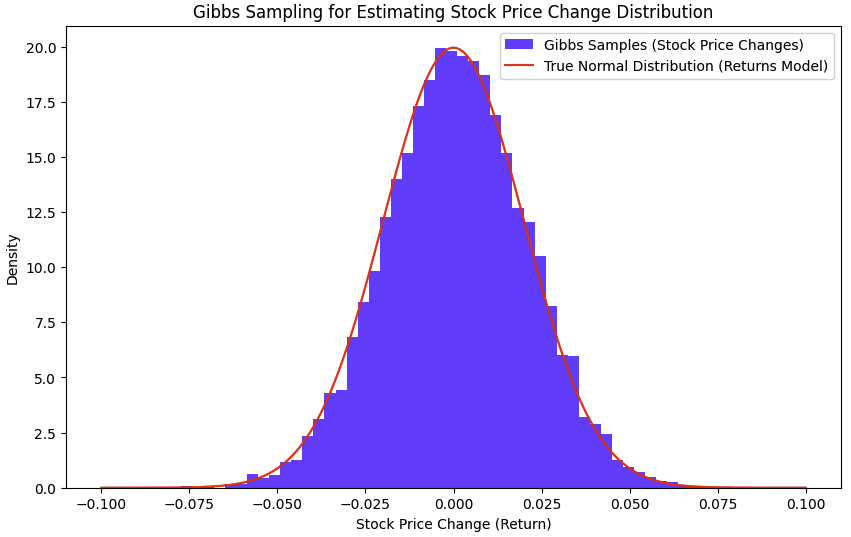
\includegraphics[width=\linewidth]{images/fig03-kuo-gibbs.png}\\[2pt]
    {\small (a) Gibbs sampling}
  \end{minipage}\hfill
  \begin{minipage}[t]{0.48\linewidth}
    \centering
    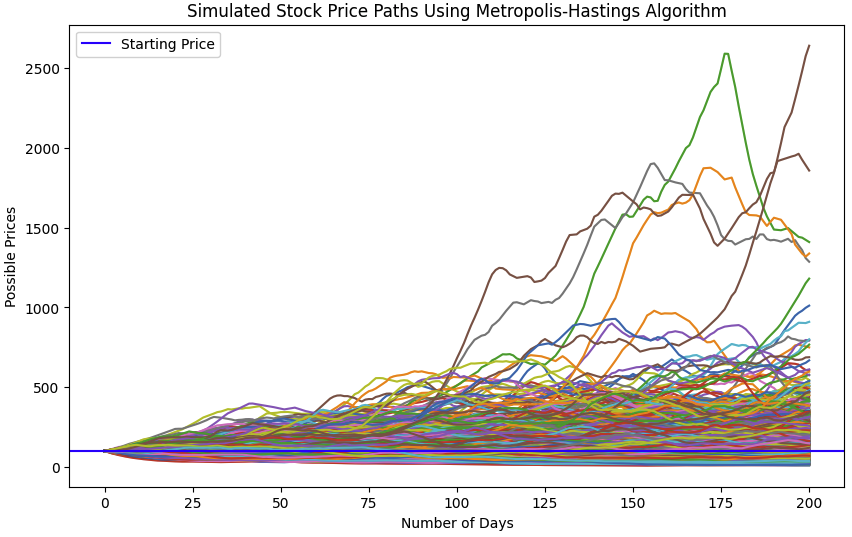
\includegraphics[width=\linewidth]{images/fig03-kuo-mh.png}\\[2pt]
    {\small (b) Metropolis--Hastings algorithm}
  \end{minipage}
  \caption{Simulated stock price paths from two MCMC algorithms, each showing 1,000 paths over 200 trading days from a starting price of \$100 (horizontal line). (a)~With Gibbs sampling, each day's return is drawn independently, and the paths spread evenly around the starting price. (b)~With the Metropolis--Hastings algorithm, each day's return depends on the previous day's, and a few paths rise far above the rest. Note the different vertical scales. Source: Kuo (2025), Figures 14.6 and 14.10.}
  \label{fig:03-mcmc-paths}
\end{figure}

The two families complement each other. The bootstrap needs no model but can show only what the sample contains. MCMC can explore outcomes that the sample never showed, but its results can be no better than the model the researcher chose.

\subsection{Multiple Testing in the Factor Zoo}
\label{sec:03-multiple}
When evaluating many candidate factors, standard cutoffs ($|t| > 1.96$) yield high false discovery rates. The reason is simple arithmetic. If 100 useless factors are each tested at the 5\% level, about five will pass by chance, and those five are the ones most likely to be written up and published. A $t$-statistic of 2 means what it says only when it is the single test that was run.

Harvey, Liu, and Zhu (2016) took the size of the search into account and recommend raising the significance threshold to $|t| > 3.0$ for new factor discoveries. The evidence supports their caution. Many published anomalies fail to clear the higher hurdle, and McLean and Pontiff (2016) found that anomaly returns fall substantially after publication, consistent with part of the original evidence being luck from the search and part being traded away once investors learned of it.

When the returns of every strategy that was tried are available, a more direct test is possible. White's (2000) \textbf{reality check}\index{White's reality check|textbf} uses the stationary bootstrap to ask how good the best of all the strategies would look by luck alone, and compares the actual winner with that benchmark. Because it resamples all strategies together, it accounts for the size of the search and for the correlations between similar strategies at the same time. Its requirement is demanding, however: it needs a record of every trial, including the ones that were abandoned. When that record does not exist, the simple hurdle of $t > 3.0$ is the practical fallback.

\subsection{Statistical vs. Economic Significance}
\label{sec:03-economic}
Statistical significance ($t$-statistic) measures precision against zero, whereas economic significance measures real-world investment impact, such as the annualized return or the improvement in Sharpe ratio, net of fees and transaction costs\index{transaction costs}. An effect is \textbf{statistically significant}\index{statistical significance|textbf} if it is unlikely to be due to chance, and \textbf{economically significant}\index{economic significance|textbf} if it is large enough to change what an investor would do. Before believing or dismissing any finding, ask two separate questions: is it real, and is it large enough to matter? Table~\ref{tab:03-stat-econ} shows that the two answers can diverge in both directions.

\begin{table}[htbp]
\centering
\small
\caption{Statistical vs. Economic Significance}
\label{tab:03-stat-econ}
\begin{tabularx}{0.9\linewidth}{@{}>{\raggedright\arraybackslash}p{0.22\linewidth}>{\raggedright\arraybackslash}X>{\raggedright\arraybackslash}X@{}}
\toprule
 & Economically Small & Economically Large \\
\midrule
\textbf{Statistically Significant} & Tiny alpha (0.4\%/yr) measured precisely in a low-risk, high-turnover portfolio consumed by trading costs. & Robust claims that survive multiple testing and cost hurdles. \\
\textbf{Not Significant} & Irrelevant finding. & Large alpha (6\%/yr) estimated imprecisely over a short, volatile sample. \\
\bottomrule
\end{tabularx}
\end{table}

Three habits keep the two questions apart. First, always report the size of an effect in units that matter, such as percent per year or a change in Sharpe ratio, alongside its $t$-statistic. Second, compare the effect with what it costs to capture: a return spread that requires monthly rebalancing of illiquid stocks may vanish after costs. Third, read a confidence interval, not just a p-value. A 95\% confidence interval is a range that would contain the true value in 95\% of repeated samples, and an interval of ``1\% to 11\% a year'' says more than ``$p = 0.02$,'' because it shows that the effect could be negligible or enormous. Harvey (2017), in his presidential address to the American Finance Association, made the same argument: researchers should combine statistical evidence with prior plausibility and economic magnitude, and no claim should survive on a $t$-statistic alone.

\section{What Investors Can Use}
\label{sec:03-investors}

Most investors will never compute a Newey--West standard error or a GRS statistic, but the ideas in this chapter translate directly into questions about any statistical claim.

\textbf{Rules of Thumb:}
\begin{enumerate}
  \item \textbf{Unbundle alpha from factor beta.} Do not pay active fees for static loadings on known factors ($SMB$, $HML$, $UMD$), because those exposures can be bought cheaply through index and factor funds.
  \item \textbf{Count independent observations.} $T$ monthly observations with a $k$-month horizon provide only about $T/k$ independent periods. Fifty years of five-year returns is ten independent observations, not six hundred.
  \item \textbf{Demand higher cutoffs.} Require $t > 3.0$ for proposed factor anomalies to adjust for search bias, and remember that across 25 portfolios one or two will look significant by chance.
  \item \textbf{Convert $t$-statistics to net returns.} Evaluate alpha after transaction costs, short-selling fees, and turnover. A significant alpha smaller than the fund's fee is worth nothing to the investor.
\end{enumerate}

\textbf{Questions to Ask Fund Managers:}
\begin{itemize}
  \item What standard errors were used, and do your results hold under Newey--West HAC and block bootstrap methods?
  \item What fraction of net performance comes from true alpha versus systematic factor exposures?
  \item How many candidate models or variations were backtested before selecting this strategy?
  \item If you forecast over long horizons, how many non-overlapping periods does your sample contain?
  \item What is the confidence interval for your alpha, and how large is it after fees and trading costs?
\end{itemize}

\section*{Exercises}
\addcontentsline{toc}{section}{Exercises}

\subsection*{Conceptual (all readers)}
\begin{enumerate}
  \item Daily returns show minimal autocorrelation, yet absolute daily returns show strong autocorrelation. Explain how both statements can be true, and why this matters for standard errors.
  \item An active equity manager reports a CAPM alpha of 3.2\% per year ($t = 2.5$). Under a Fama--French three-factor model, the alpha drops to 0.1\% ($t = 0.2$), with an $SMB$ loading of 0.70 and an $HML$ loading of 0.50. Explain the source of the manager's excess return, and what it implies for the fee the manager should charge.
  \item A long-horizon regression of 5-year returns on dividend yields uses 50 years of monthly data ($T=600$, $k=60$). How many independent observations does it contain, and why are classical $t$-statistics misleading?
  \item Why must a time-series bootstrap resample blocks of observations rather than individual months?
  \item Explain why a factor alpha with $t = 3.2$ might lack economic significance, and list what you would need to know before investing in it.
  \item A stock has a market beta of 0.8, a residual standard deviation of 6\% a month, and the market's standard deviation is 4.5\% a month. Use Equation~\eqref{eq:03-vardec} to compute the share of its variance that is systematic. What would the share be for an equally weighted portfolio of 50 such stocks with independent residuals?
\end{enumerate}

\subsection*{Lab Extensions (technical readers)}
\begin{enumerate}
  \setcounter{enumi}{6}
  \item Replicate Part B of Lab~\ref{ch:03} across two sub-samples: 1963--1992 and 1993--present. Compare changes in factor risk premia and GRS test rejections.
  \item Compute $t$-statistics for 25 portfolio alphas using four methods: Classical OLS, White, Newey--West, and Stationary Block Bootstrap. Identify portfolios with the largest SE discrepancies, and explain what features of their returns might cause them.
  \item Pair monthly returns with 1,000 simulated non-predictive predictors ($\rho = 0.98$). Run long-horizon regressions ($k=1$ to $60$) and plot false-positive rates for OLS, Newey--West, and Hodrick standard errors. Then set the correlation between predictor shocks and return shocks to $-0.9$ and describe how the Stambaugh bias changes the results.
\end{enumerate}

\section{Lab~\thechapter: Replicating Fama and French (1993) and Testing Robust Standard Errors}
\label{sec:03-lab}

\begin{callout}
\noindent \textbf{Lab~\ref{ch:03} at a Glance.} \emph{Claim on trial:} Variation in expected stock returns can be explained by systematic risk factors, and regression statistics remain reliable once standard errors account for non-Gaussian features. \emph{Data:} 25 Fama--French portfolios formed on Size and Book-to-Market plus factor returns ($R_m-r_f$, $SMB$, $HML$) and daily market returns from the Kenneth French Data Library\index{Kenneth French data library}, downloaded automatically. \emph{Tools:} Python with pandas, NumPy, SciPy, and matplotlib. \emph{Code:} \texttt{ch03-noisy-returns/}.
\end{callout}

The lab repeats the logic of several landmark studies with free data, so that you can see each result for yourself. Part A measures the stylized facts of Section~\ref{sec:03-facts}. Part B replicates the regressions of Fama and French (1993) and decomposes each portfolio's risk. Part C tests the model jointly and compares four standard errors. Part D is a controlled experiment in which the truth is known, so we can see exactly how often each method is fooled.

\subsection*{Lab Structure}

\textbf{Part A: Stylized Facts.} The lab computes the mean, variance, skewness, and kurtosis of daily and monthly market returns and of each of the 25 portfolios. It counts extreme tail events beyond $3\sigma$ and compares the count with what a normal distribution would predict, and it plots the autocorrelations of returns and of absolute returns. Expect returns themselves to show little memory and their absolute size to show a great deal: volatility clustering in one picture.

\textbf{Part B: Multi-Factor Regressions and Risk Decomposition.} The lab estimates the CAPM and the Fama--French three-factor regressions, Equations~\eqref{eq:03-capm-ts} and~\eqref{eq:03-ff3}, for all 25 portfolios from July 1963 onward. It reports each portfolio's loadings, alpha, and $R^2$ under both models, and it splits each portfolio's variance into systematic and idiosyncratic parts with Equation~\eqref{eq:03-vardec}. It also runs the Fama--MacBeth procedure of Equation~\eqref{eq:03-fmb} to estimate each factor's risk premium. Expect $R^2$ to rise substantially from the CAPM to the three-factor model, above 90\% for most portfolios, and the alphas to shrink toward zero. This \textbf{alpha decay} is the risk decomposition at work: returns that the CAPM leaves unexplained are reassigned to exposures to size and value.

\textbf{Part C: Multivariate Tests and Standard Error Comparison.} The lab runs the GRS test of Equation~\eqref{eq:03-grs} across all 25 portfolio intercepts under each model and checks its p-value with a bootstrap. It then computes four $t$-statistics for each alpha (Classical, White, Newey--West, and Stationary Bootstrapped) and reports how many alphas are significant under each method. Expect the GRS test to reject the CAPM decisively. The three-factor model fits far better, but it is often rejected too, mostly because a few portfolios, such as the smallest growth stocks, keep sizable alphas. Expect also that the four standard errors agree closely, because monthly portfolio returns have little autocorrelation and no overlap. That agreement is itself a finding: robust standard errors are cheap insurance, not a guarantee of different answers.

\textbf{Part D: Controlled Overlapping Regression Experiment.} The lab regresses real market returns on 1,000 simulated non-predictive persistent predictors ($\rho=0.98$) for horizons $k=1$ to $60$, using Equation~\eqref{eq:03-overlap}. Because the predictors have no predictive power by construction, a correct 5\% test should reject about 5\% of the time at every horizon. The lab compares rejection rates across OLS, Newey--West, and Hodrick standard errors and plots the average $R^2$ of these useless predictors. Expect OLS to reject far more often as the horizon grows, Newey--West to do better but still reject too often at long horizons, Hodrick to stay close to 5\%, and the average $R^2$ to rise with the horizon even though there is nothing to find.

\emph{[Draft note: the figures and numbers for Parts A to C, and the real-return inputs to Part D, are generated from the Kenneth French data at the time of publication. The text above describes what theory and earlier studies predict.]}

\subsection*{Verdict}
\textbf{Survives, with conditions.} Each half of the claim holds, but only under conditions that the lab makes visible.
\begin{enumerate}
  \item \textbf{Factors explain most of the variation, but not all of the average returns.} Multi-factor models capture substantial variation in diversified portfolios ($R^2 > 90\%$), so a few systematic factors do describe most of their risk. The GRS test can still reject the model, which shows that a high $R^2$ is not the same as zero alphas.
  \item \textbf{For non-overlapping monthly data, the statistics are reliable.} Standard error choices make little difference, because classical, White, Newey--West, and bootstrap standard errors usually agree.
  \item \textbf{For overlapping horizons or persistent predictors, classical statistics fail severely.} Standard analytical standard errors find far too many false discoveries, and valid inference requires Hodrick standard errors or block bootstrapping.
\end{enumerate}
The lesson is a rule you can apply to any regression. Match the factor model to the risks the investment actually took, match the standard error to the design of the study using Table~\ref{tab:03-se-guide}, and report the size of the effect alongside its $t$-statistic.
